\documentclass[document.tex]{subfiles}
\begin{document}

\chapter{Feature Selection and Classification}
\noindent Feature mining generally refers to transform a high dimensional correlated dataset into a low dimensional uncorrelated data space. It can be done by following two steps:
\begin{itemize}
	\item Feature extraction
	\item Feature selection
\end{itemize}

\section{Feature Extraction Based on Principal Component Analysis}
\noindent Principal component analysis (PCA)\cite{7} is one of the most popular unsupervised feature extraction technique.The principal component analysis is based on the fact that neighboring bands of hyperspectral images are highly correlated and often convey almost the same information about the object. The PCA employs the statistic properties of
hyperspectral bands to examine band dependency or correlation. This transformation
is based on the mathematical principle known as eigenvalue decomposition of the
covariance matrix of the hyperspectral image bands to be analyzed. The new transformed uncorrelated variables called principal components (PCs). First few variable contains most of the variation of the original data. If a hyperspectral image form M = i * j * k dataset where i is number of rows, j is number of columns and k is the number of bands of the dataset. Then after applying PCA to our dataset, we can use a small portion of k and still find almost all variations of our data. $X_1,X_2,X_3,....,X_n$ is the bands of the dataset. 
\begin{figure}[H]
	\begin{center}
		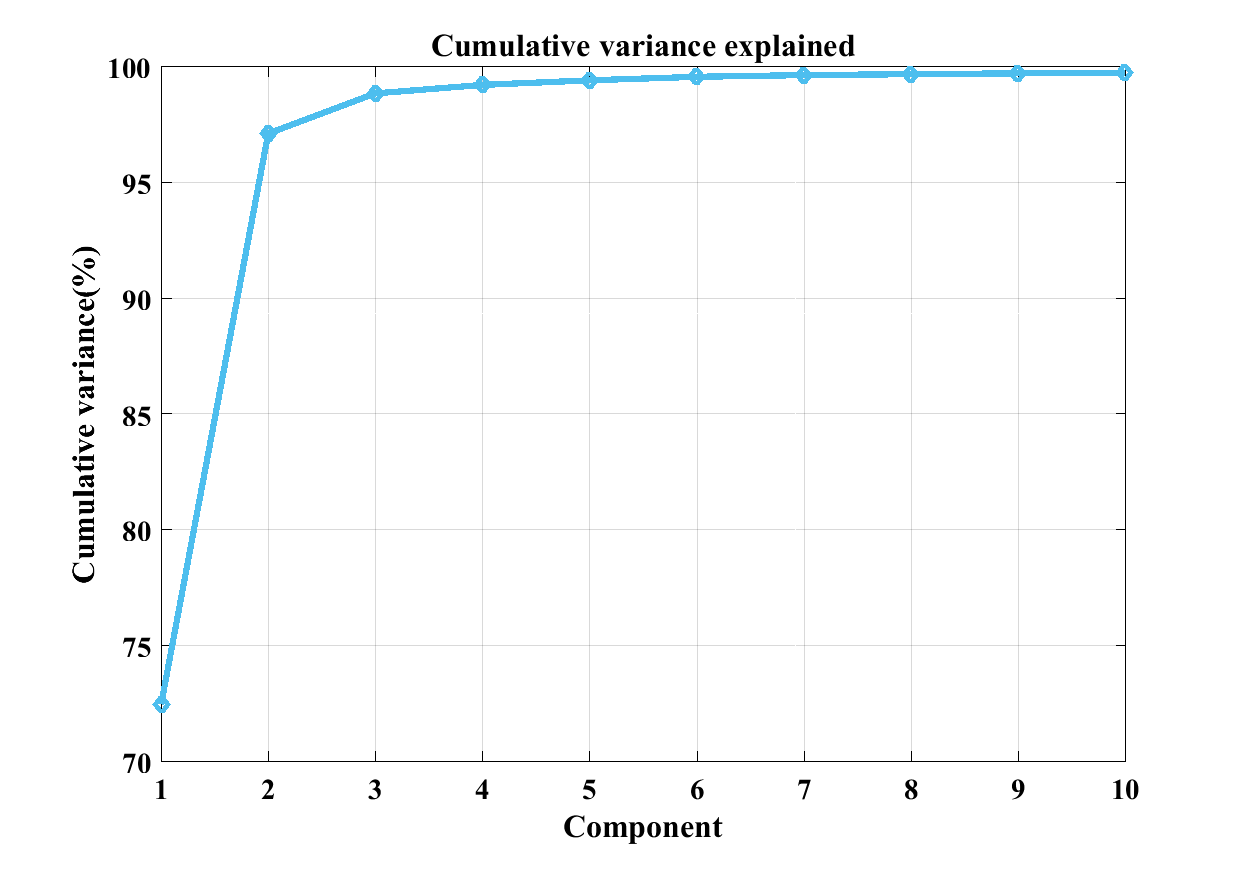
\includegraphics[height=8.0cm]{imgs/variance.png}
	\end{center}
	\caption{Cumulative variance of bands obtained via PCA}
	\label{fig:Cumulative variance of bands obtained via PCA}
\end{figure}
\noindent For calculating PCA we first subtract mean form the dataset. The mean is calculated as
\begin{equation}
\overline{X} = \dfrac{\sum_{i=1}^{n} X_i}{n}
\label{eq:Mean}
\end{equation}
The covariance matrix between any two dimension can be calculated as:
\begin{equation}
COV(X,Y) = \dfrac{\sum_{i=1}^{n}(X_i - \overline{X})(Y_i - \overline{Y})}{n-1}
\end{equation}
Covariance matrix is a square matrix. Eigenvalue and eigenvector is calculated from covariance matrix. Eigenvector that has the highest eigenvalue is the first principal component. Arrangement of eigenvectors according to descending order of eigenvalues creates a matrix of new set of data whose first few column can be chosen for further use.
 
\section{Feature Selection Based on Normalized Mutual Information}
\noindent Mutual Information (MI) measures the amount of information one random variable holds about the other random variable\cite{20} by quantifying dependencies of those variables. Mutual information of two random varibles X and Y can be defined as:
\begin{equation}
I(X,Y) = \sum_{y=1}^{L1}\sum_{x=1}^{L2}p(x,y)\log\dfrac{p(x,y)}{p(x)p(y)}
\end{equation}
where x, y are the pixel values and L1, L2 are the maximum
pixel values of the input images. P(x,y) is joint probability distribution function and P(x) and P(y) is marginal probability distribution function of variable X and Y respectively. If two variable x and
y are independent, x does not know any information about y and vice versa. So their
mutual information will be zero. According to Shannon’s information theory, if the
probability of a random variable x is P(x) then uncertainty of x measured by entropy\cite{20} is:
\begin{equation}
H(x) = -p(x)log(p(x))
\end{equation}
Here mutual information can also be described as:
\begin{equation}
I(X,Y) = H(X) + H(Y) - H(X,Y)
\end{equation}
Where H(A) and H(B) are the entropies of A and B and H(A,B)
is their joint entropy. Now by calculating mutual information between class label $c = c_1,c_2,....c_N$ and bands $f = f_1,f_2,...f_N$ of the hyperspectral image we can select relevant features for classification. Each feature will be selected in descending order $I_1 \geq I_2 \geq I_3 \geq....\geq I_N$. Feature with highest mutual information contains most information. It is difficult to use the value given by (4.3) directly in an absolute sense, as it is affected by the entropy of the two variables and not bounded to [0, 1]. A few methods to normalize mutual information are available to give a new value between 0 and 1, where 0 is the value for the independent case and 1 for the identical or one-to-one relationship case. Normalized mutual information (nMI)\cite{21} is defined as follows:
\begin{equation}
\hat{I}(X,Y) = \dfrac{I(X,Y)}{\sqrt{I(X,X)}\sqrt{I(Y,Y)}}
\end{equation}

\subsection{Original Dataset Plus nMI Approach}
\noindent In feature selection, the relevant features have important
information required to produce the classification output. The aim of feature selection is to find only informative features $k < n$ for a dataset. If the reference image is f and original dataset is x then the normalized mutual information between f and x is given below:
\begin{equation}
\hat{I}(x_i,f_j) = \dfrac{\sum_{i}\sum_{j} p(x_i,f_j)\log\dfrac{p(x_i,f_j)}{p(x_i)p(f_j)}}{\sqrt{I(x_i,x_i)}\sqrt{I(f_j,f_j)}}
\end{equation}  

\subsection{PCA Dataset Plus nMI Approach}
\noindent In order to find informative features from the transformed features
obtained by unsupervised feature extraction technique principal component analysis (PCA) normalized mutual information (nMI) is applied as below. If the reference image is f and PCA transformed dataset is y then the normalized mutual information between f and y is given below:
\begin{equation}
\hat{I}(y_i,f_j) = \dfrac{\sum_{i}\sum_{j} p(y_i,f_j)\log\dfrac{p(y_i,f_j)}{p(y_i)p(f_j)}}{\sqrt{I(y_i,y_i)}\sqrt{I(f_j,f_j)}}
\end{equation}  

\section{Proposed Method}
\noindent The proposed method is a target class oriented feature selection technique which select relevant features for each class of the dataset using principal component analysis (PCA) as feature extraction\cite{7} and normalized mutual information (nMI) as features selection\cite{9}. At first, the unsupervised feature extraction technique PCA is applied to find uncorrelated dataset in smaller data space. Then normalized mutual information (nMI) with two constraints to maximize general relevance and minimize redundancy on the components obtained via PCA is applied for feature selection\cite{21}. Here we consider one class of the dataset at a time and make all others as the background class. For each class of the dataset feature selection method is applied to obtain a relevant feature space to classify that class. Finally kernel support vector machine (SVM) is applied for classification purpose of the data set\cite{11}. Here first SVM use those selected features of each class to train a model for that specific class and test data to find test result for that specific class. RBF kernel\cite{22} is used in SVM as the relationship between class label C and datase $X_i$ is nonlinear. K-fold cross validation is applied to find correct parameter C and $\gamma$ of KSVM for each target class of the dataset. Finally average of those accuracy for each class is the final classification accuracy.

\section{Implementation}

\subsection{Implementation of PCA Based Feature Extraction}

\subsection{Implementation of nMI Based Feature Selection}

\subsection{Implementation of Target Class Oriented Feature Selection}

\section{Experimental Results}

\subsection{Indian pines (92AV3C) Dataset}
\subsection{Feature Extraction Result}
\subsection{nMI Based Feature Selection Result}
\subsection{Target Class Oriented Feature Selection Result}
\section{Classification Results}
\end{document}